\documentclass[12pt]{article}
\usepackage{lingmacros}
\usepackage{tree-dvips}
\usepackage{graphicx}
\usepackage{ragged2e}
\usepackage{comment}
\graphicspath{{./images/}}
\setlength{\parindent}{4em}
\setlength{\parskip}{1em}
\begin{document}
\title{Documentazione Ingegneria del Software}
\author{Silviu Filote, Simone Ronzoni, Jonathan Bommarito, Nicolò Carissimi}
\date{January 25, 2022}
\maketitle % titolo
\pagenumbering{arabic}


\tableofcontents
\newpage
\raggedright

\section{Software Life Cycle}
Per il progetto si è deciso di utilizzare il modello Agile Scrum. Siccome non vi è la necessità di comunicare volta per volta con il cliente, ad ogni sprint verrà eletto un product owner tra i diversi componenti del gruppo che avrà il compito di:
\begin{itemize}
  \item pianificare il lavoro per lo sprint corrente;
  \item assicurarsi che le task completate siano state chiuse;
\end{itemize}
\section{Configuration Management}
Il sistema di configuration management utilizzato è GitHub, sia per la \newline 
creazione dei task che per il versioning del codice. \newline
Per quanto riguarda la creazione dei task, partendo dalle note presenti nel Backlog, si creano gli Issue che si decide di implementare per lo sprint corrente e vengono assegnati ad un membro del team. \newline
Per la gestione e il monitoraggio dell'avanzamento degli issue viene usato il project board presente su GitHub con il template "Basic kanban". \newline
Per il completamento di ogni task si è utilizzata la seguente modalità:
\bigskip
\bigskip
\begin{itemize}
  \item Creazione del branch utilizzando come naming convention il numero progressivo del task
  \item Implementazione del codice necessario per completare il task
  \item Aggiunta e commit delle modifiche sul proprio branch locale
  \item Push branch da origin a remote 
  \item Push modifiche sul branch remoto
  \item Apertura merge request verso main 
  \item Assegnazione review e compilazione merge request
  \item Approvazione dei reviewers
  \item Merge
  \item Cancellazione branch remoto e locale
\end{itemize}
\begin{figure}[ht]
  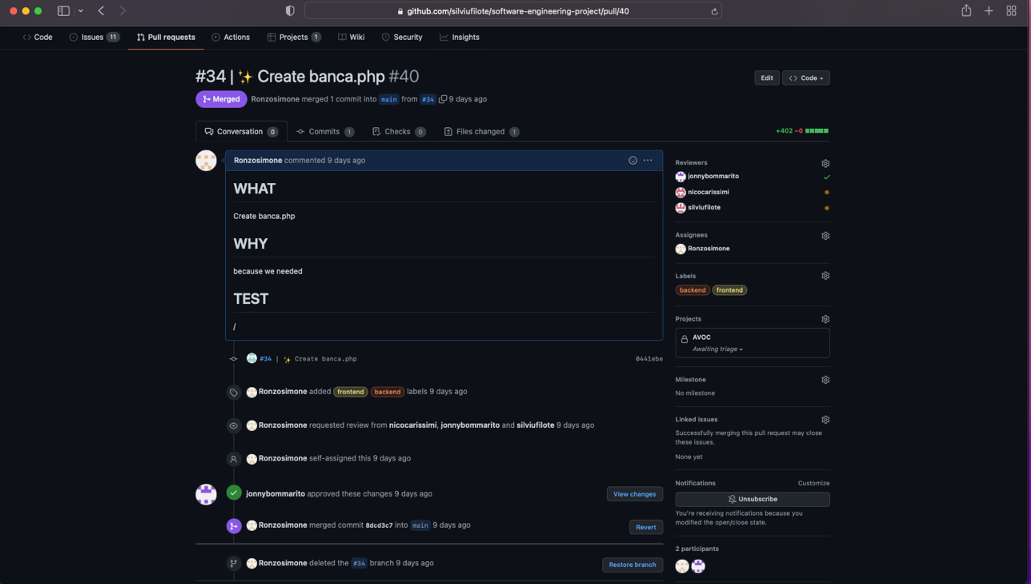
\includegraphics[width=1.2\textwidth]{mergeRequest.png}
  \caption{Merge Request tipica su GitHub}
\end{figure}
\section{People Management and Team Organization}
Siccome nel progetto si è utilizzato un approccio agile, l'organizzazione all'interno del team non ha una rappresentazione rigida.
Nel caso in cui si palesino difficoltà, queste vengono esposte nello stand up meeting, chiarite e, se necessario, vengono schedulate delle sessioni di Pair programming.

\pagebreak
\section{Requirement Engineering}

\begin{enumerate}
  \item\textbf{\large Introduction} 
  \begin{enumerate}
    \item\textbf{Purpose} \newline
    Avoc è un web app realizzata per il concessionario Boninsegna s.r.l. che consenta ai clienti di richiedere un preventivo per comprendere la convenienza tra un noleggio e un leasing, consentendo un'eventuale sottoscrizione.
    \item\textbf{Scope} \newline
    Il prodotto che si vuole realizzare automatizza le funzionalità descritte nel punto precedente.
  Lo scopo del servizio è di agevolare i clienti del concessionario attraverso le funzionalità offerte online.
  Questo permetterà di estendere la clientela passando dai soli utenti locali, ad un bacino più ampio.
    \item\textbf{Definitions, acronyms and abbreviations} \newline
    Admin: per admin ci si riferisce ad un dipendente del concessionario che possiede il privilegio di aggiungere, rimuovere o modificare macchine. \\
    Utente: per utente si intende un qualsiasi utilizzatore del sito che non sia admin.
    \item\textbf{Overview} \newline
    Nella sezione 2 si trova un overview generale del sistema, nella sezione 3 vengono invece descritti i requisiti funzionali e non funzionali.

    
  \end{enumerate}
  \newpage
  \item\textbf{\large Overall description} 
   \begin{enumerate}
    \item\textbf{Product perspective} \newline
    Si utilizza il database già presente all'interno dell'organizzazione, contenente tutte le informazioni relative alle vetture, e si aggiunge la tabella relativa agli utenti e quella relativa finanziamenti che essi stipulano.
    \bigskip
    \item\textbf{Product functions} \newline
    \begin{itemize}
     \item Funzionalità per visualizzare macchine e sottoscrivere contratti per l'utente;
     \item Funzionalità di gestione del parco macchine per gli admin;
    \end{itemize}
    \bigskip
    Le funzionalità vengono esposte in automatico, in base al tipo di utenza inserita in fase di login.
    \item\textbf{Constraints} \newline
    Gli utenti possono solo richiedere un preventivo e visualizzare i finanziamenti sottoscritti,
    non sono abilitati ad eseguire modifiche relative alle auto.
  \end{enumerate}
  \item\textbf{\large Specific requirements} 
  \begin{enumerate}
    \item\textbf{Hardware interfaces} \newline
    L'interfaccia utente è responsive, così che possa adattarsi alla dimensione dello schermo di qualsiasi dispositivo.
    \item\textbf{Software interfaces} \newline
    La connessione al database è stata possibile tramite l'extension mysqli.
    \newpage
    \item\textbf{Functional requirements} \newline
    \begin{enumerate}
      \item{USER}
    \begin{itemize}
      \item{SignIn} \newline
    
      \smallskip
      L'utente ha a disposizione una finestra di dialogo dove inserire i parametri per effettuare il login.
      i suddetti parametri sono il codice utente e la propria password. \\
      In caso quest'ultimo sia andato a buon fine, l'utente sarà stato correttamente loggato
      \smallskip
      \item {SignUp} \newline
      
      \smallskip
      L'utente ha a disposizione una finestra di dialogo dove inserire i parametri per effettuare la registrazione tra cui:
      \begin{itemize}
        \item{Nome}
        \item{Cognome}
        \item{CodiceFiscale}
        \item{DataDinascita}
        \item{E-mail}
        \item{Password}
      \end{itemize}
      \bigskip
      \item {CalcolaFinanziamento} \newline
      
      \smallskip
      
      L'utente può scegliere dal menù a tendina il brand, il modello e la versione di una macchina presente nel concessionario.
      Successivamente viene calcolato il prezzo e viene evidenziato il button per la configurazione del finanziamento.
      Attraverso la modale sono richiesti i seguenti parametri:
      \begin{itemize}
        \item{Tipologia}
        \item{RataMensile}
        \item{Anticipo}
        \item{Chilometreggio}
      \end{itemize}
      \end{itemize}
      \newpage
    \item{ADMIN}
    \smallskip
    \begin{itemize}
      \item{SignIn} \newline
      
      \smallskip
      L'admin ha a disposizione una finestra di dialogo dove inserire i parametri per effettuare il login tra cui il codice utente e la propria password.
      In caso quest'ultimo sia andato a buon fine, l'utente sarà stato correttamente loggato con privilegi amministratore

      \smallskip

      \item {gestisci Macchine}  \newline
      

      All'interno di questa view è possibile eseguire le seguenti operazioni:

      \smallskip
      \begin{itemize}
        \item{inserimento Macchina} \newline
         
        \smallskip
          
        
           Per questa funzione viene visualizzata una modale che permette l'inserimento delle nuove auto.
           i parametri richiesti sono:
           \smallskip
           \begin{itemize}
           \item marca 
           \item modello
           \item versione
           \item AnnoImmatricolazione
           \item prezzo
           \item peso
           \item lunghezza
           \item largezza
           \item posti
           \end{itemize}
           \smallskip
           \smallskip
           \item{Modifica Macchina} \newline
           Per questa funzione è necessario cliccare sul campo che si vuole modificare e confermare attraverso il pulsante 'Modifica'
        \smallskip
        \newpage
        \item{Elimina Macchina} \newline
        
          \smallskip
           Per questa funzione è necessario cliccare sull'apposito pulsante dedicato nella colonna 'Azioni' della tabella dei record delle macchine.  
           
        \smallskip
        
        
      \end{itemize}
      \smallskip
      
      \end{itemize}
  \end{enumerate}

  \end{enumerate}
\end{enumerate}
\bigskip
\section{Software Architecture}
\begin{figure}[ht]
  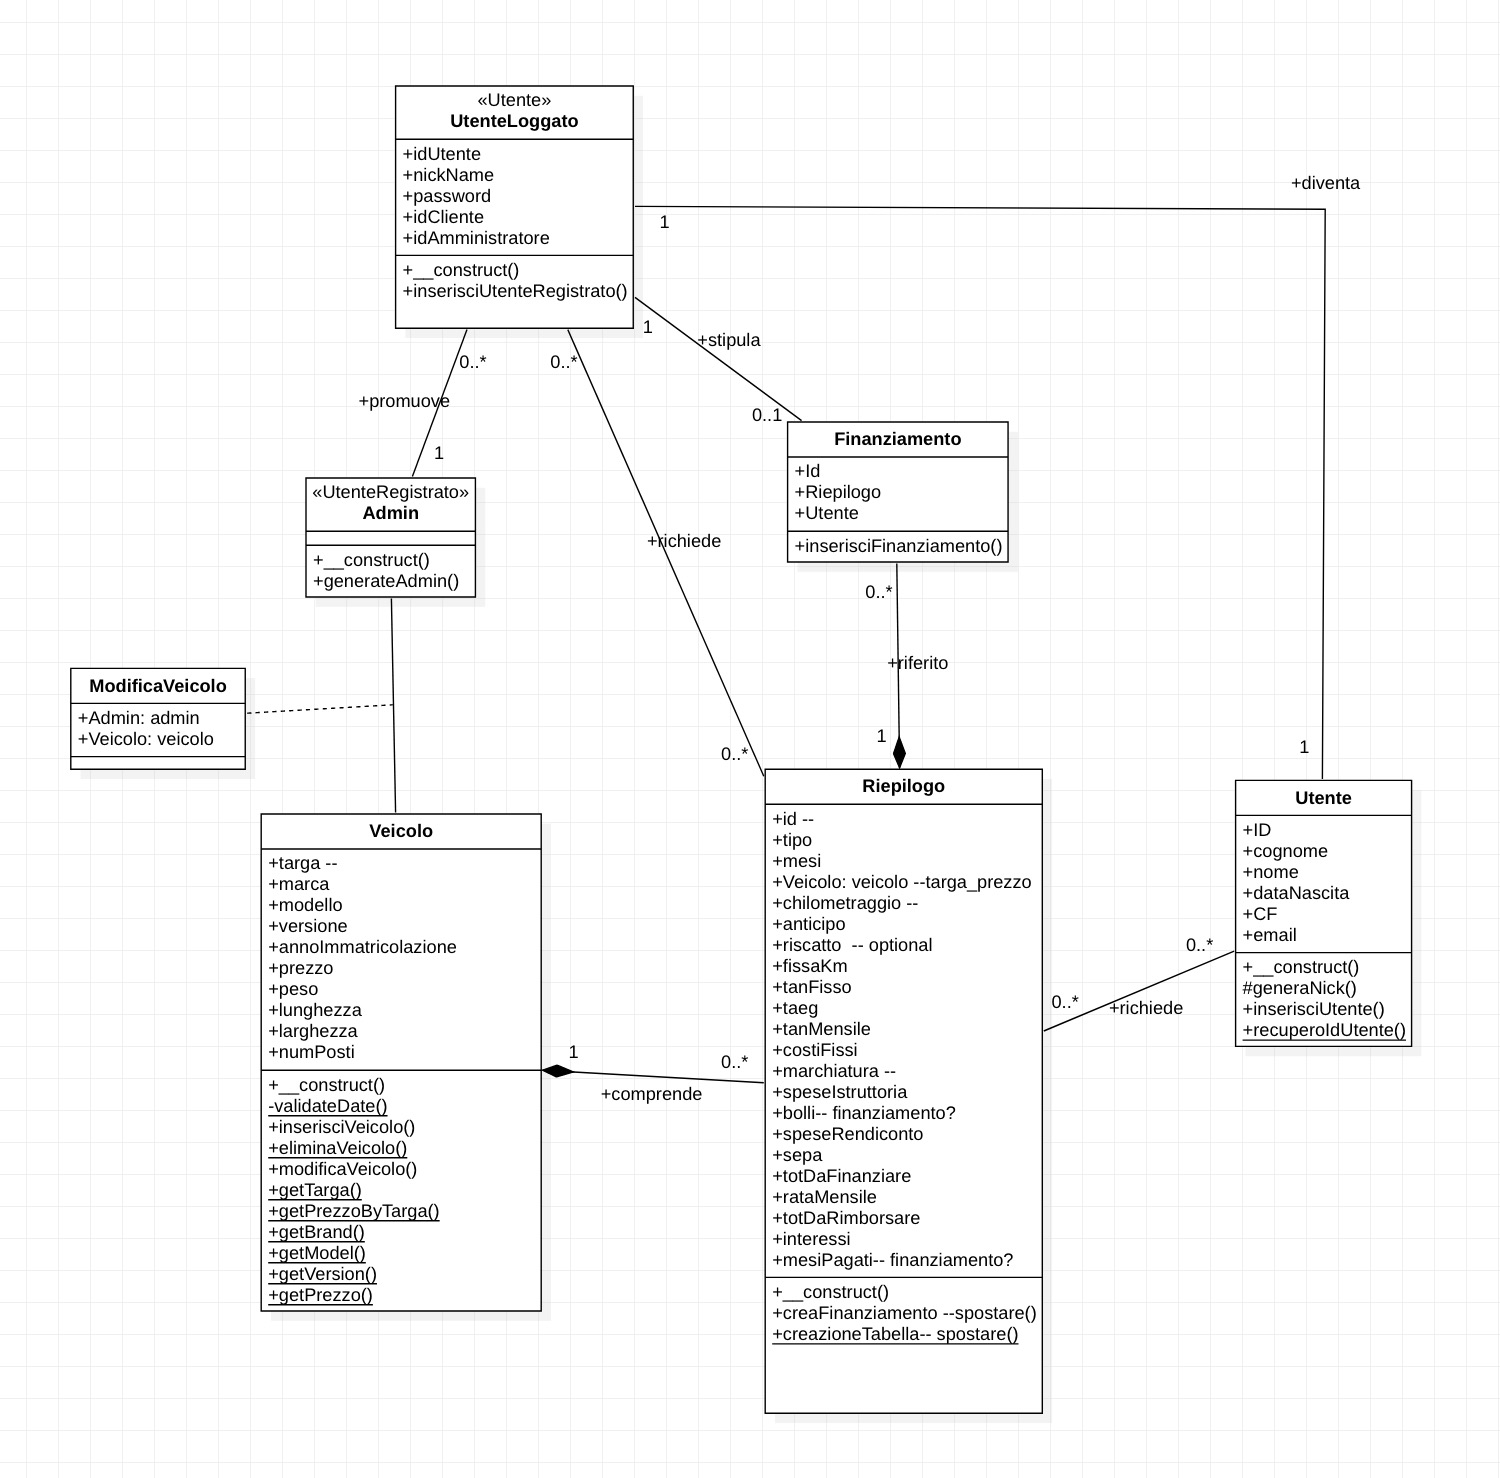
\includegraphics[width=0.90\textwidth]{ClassDiagram.jpeg}
\end{figure}
\pagebreak
\begin{figure}[ht]
  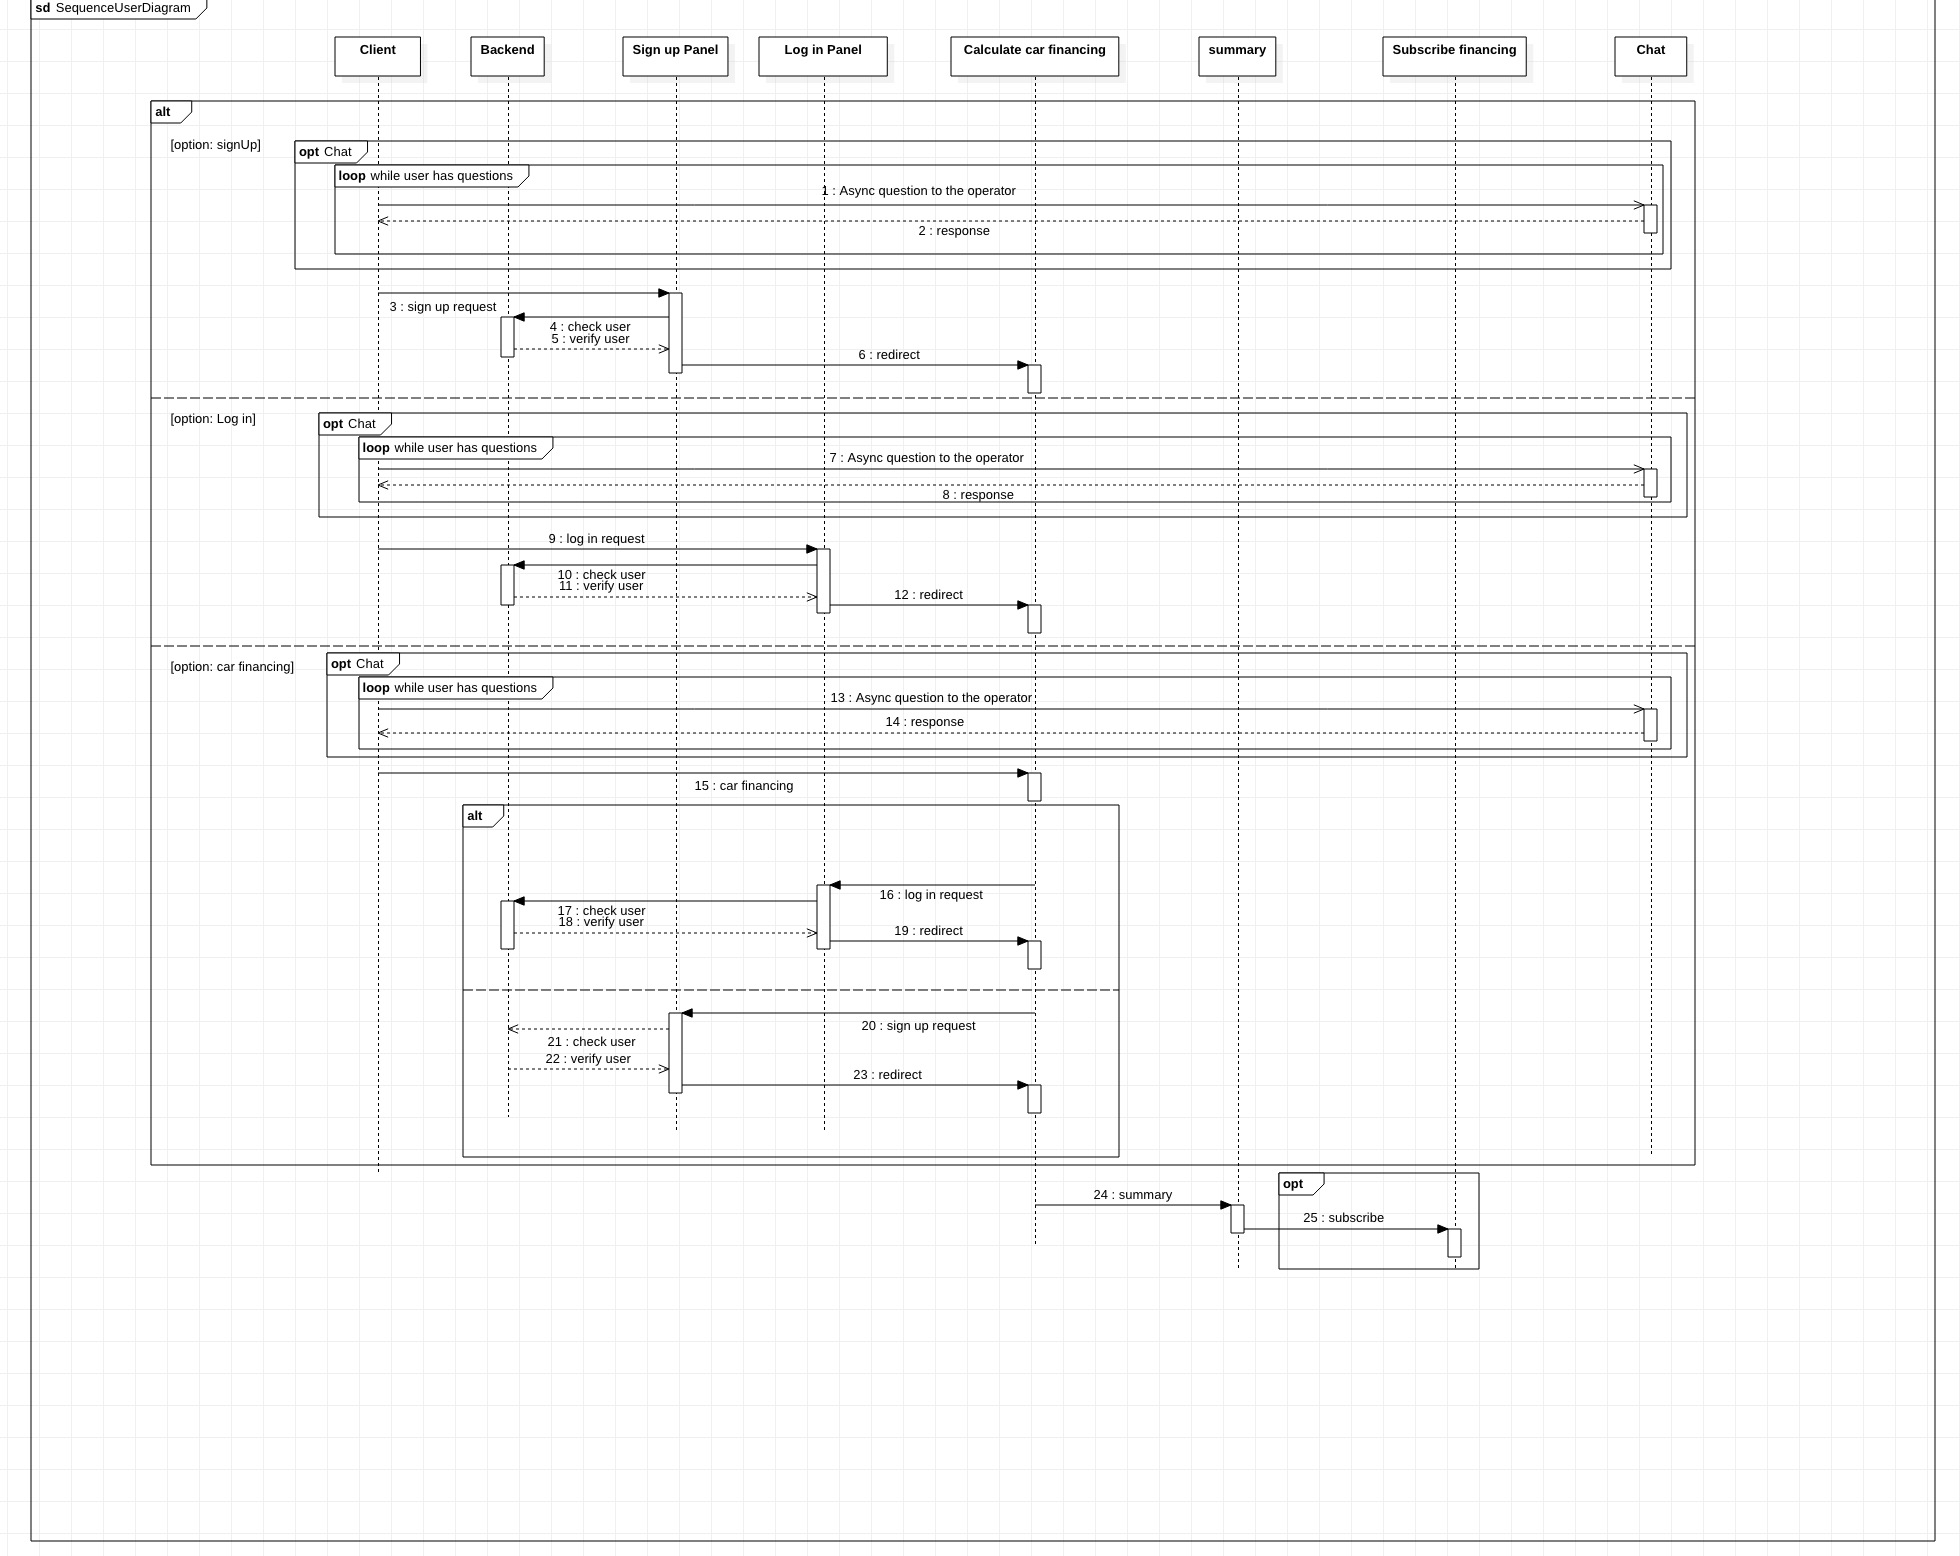
\includegraphics[width=1.20\textwidth]{Sequence.jpeg}
\end{figure}
\pagebreak  
\section{Software Design}
  \begin{center}
    DESIGN PATTERN
  \end{center}


\textbf{Delegation:} \\ 
La classe admin è in grado di utilizzare tutte le funzioni della classe veicolo, tra cui:
\begin{itemize}
  \item aggiungi veicolo;
  \item elimina veicolo;
  \item modifica veicolo;
\end{itemize}

\section{Software Testing}
{Test documentation based on IEEE 928} \\
\begin{itemize}
\item \textbf{Test plan}: \\ il piano di test consiste nell’importare tutte le classi con le relative dipendenze e testare tutti i metodi cercando di ottenere la massima copertura possibile. 

\item \textbf{Test design specification:} \\ i nomi dei componenti richiamano le funzionalità che svolgono
\begin{itemize}
  \item Admin.php 
  \item Riepilogo.php
  \item Utente.php
  \item UtenteRegistrato.php 
  \item Veicolo.php
\end{itemize}
\item  \textbf{Test procedure specification:} \\
Se i metodi sono statici vengono richiamati passando gli opportuni parametri, per i metodi non statici vengono creati degli oggetti di supporto.

\item \textbf{Test item transmittal report:} \\
Gli elementi testati si trovano nella cartella ./classi e verranno testati tutti i metodi all’interno degli stessi.
\item \textbf{Test log:} \\
Testing a partire dalle classi meno popolate fino ad arrivare a quelle più complesse. 

\item \textbf{Test incident report:} \\
Nulla da trasmettere.
\item \textbf{Test summary report:} \\
I test sono stati esaustivi e hanno evidenziato alcuni importanti bug.
\end{itemize}


\section{Software Maintenance}

Le attività di Refactor sono state le seguenti:
\begin{itemize}
  \item Refactor della homepage suddividendola in più moduli per favorire la granularità;
  \item Introduzione del PDO nelle query al fine di migliorare la sicurezza;
  \item Gestito il redirect tramite .htaccess;
\end{itemize}



\end{document}